	Este manual pretende describir el funcionamiento de la aplicación \textit{DIRe}, esta aplicación tiene como finalidad realizar los cálculos necesarios para el diseño de reactores ideales.
	
	Esta aplicación se ha desarrollado usando Python 3, la interfaz gráfica se ha creado con el programa \textit{Qt Designer} y se ha transformado a Python para que sea compatible con la librería \textit{PySide 1.2.4}. 
	
	Pues que la librería \textit{PySide 1.2.4} no es compatible con Python 3.5, se usará Python 3.4. Es posible usar la versión 3.5 si se tiene instalado la \textit{PySide 2}.
	
	Para el correcto funcionamiento de la aplicación es necesario tener los siguientes módulos instalados:
	\begin{itemize}
		\item Pyqtgraph para poder visualizar gráficas dentro de la aplicación Qt.
		\item Matplotlib para poder visualizar y exportar los resultado de los cálculos.
		\item Scipy permite realizar las distintas operaciones matemáticas.
		\item Numpy proporciona las clases necesarias para operar con vectores.
	\end{itemize}
	
	%\newpage
	
	La aplicación está dividida en distintas ventanas según se verá a lo largo de este documento.
	
\section{Ventana principal y ventana de selección}
	La primera ventana que aparece al ejecutar la aplicación se puede ver en la Figura \ref{vent_prin}. Desde esta ventana se pueden realizar las siguientes acciones:
	\begin{itemize}
		\item Acceder a la ventana de selección del reactor.
		\item Salir de la aplicación.
		\item Visualizar la guía de usuario de la aplicación, en esta guía se muestran las ecuaciones usadas para el diseño de los reactores y los parámetros necesarios. Ver Figura \ref{vent_ayuda}
	\end{itemize}

	\begin{figure}[!h]
		\centering
		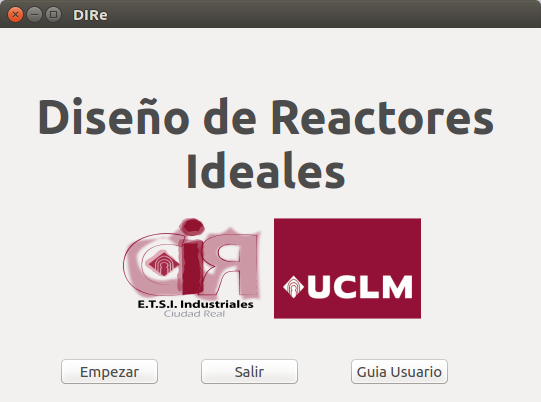
\includegraphics[width=0.8\textwidth]{./imagenes/DIRe_051.png}
		\label{vent_prin}
		\caption{Ventana Principal}
	\end{figure}
	
	\begin{figure}[!h]
		\centering
		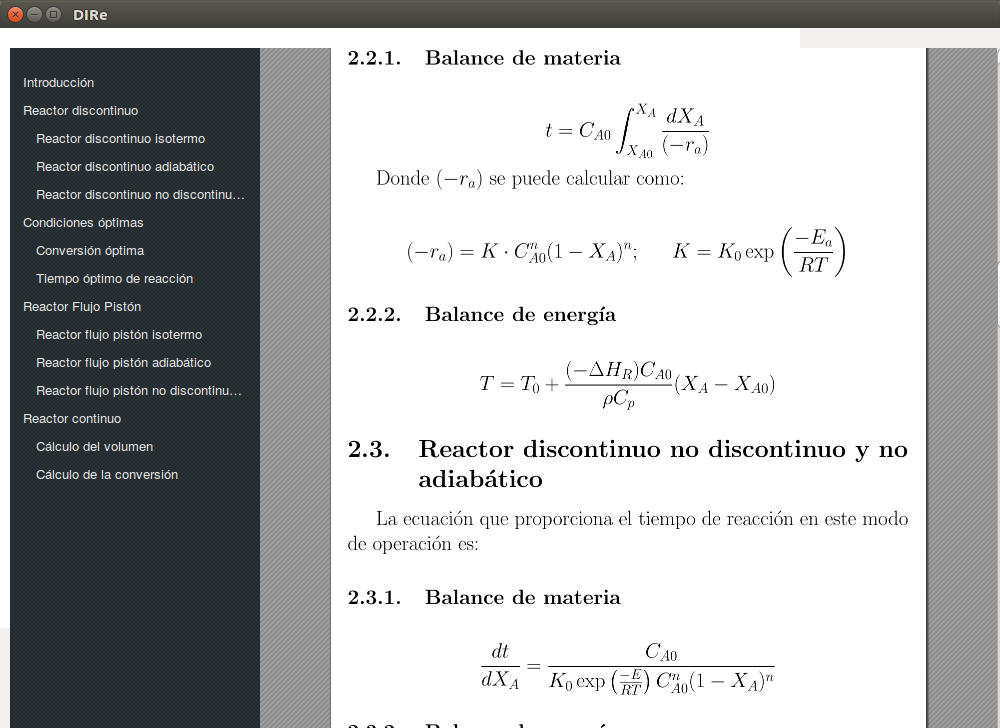
\includegraphics[width=0.8\textwidth]{./imagenes/DIRe_050.png}
		\label{vent_ayuda}
		\caption{Ventana de ayuda}
	\end{figure}

	En la ventana de selección se muestran botones que permiten seleccionar entre los distintos tipos de reactores. Los reactores que se pueden calcular son:
	
	\begin{itemize}
		\item Reactores discontinuos, dentro de este tipo se divide en isotermos, adiabáticos y otro tipo que no es ni adiabático ni isotermo.
		\item Reactores continuos (flujo pistón), dentro de este tipo se divide en isotermos, adiabáticos y otro tipo que no es ni adiabático ni isotermo.
		\item Reactores de lecho fijo.
	\end{itemize}

	En la Figura \ref{vent_seleccion} se puede ver la ventana de selección.
	
	\begin{figure}[!h]
		\centering
		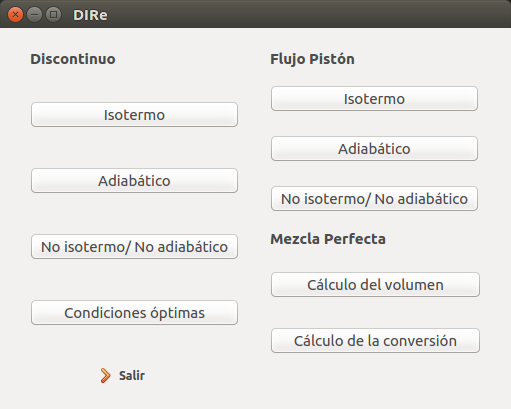
\includegraphics[width=0.8\textwidth]{./imagenes/DIRe_060.png}
		\label{vent_seleccion}
		\caption{Ventana de selección}
	\end{figure}

